\documentclass{beamer}

\usepackage{amsmath}
\usepackage{graphicx}
\usepackage{bm}
\usepackage{fontawesome}
\usepackage{colortbl}
\usepackage{mathtools} 
\setbeamerfont{normal text}{size=\small}

% tikz
\usepackage{tikz}
\usetikzlibrary{%
  arrows,%
  backgrounds,
  intersections,
  shapes,
  shapes.misc,% wg. rounded rectangle
  shapes.arrows,%
  chains,%
  matrix,%
  positioning,% wg. " of "
  scopes,%
  decorations.pathmorphing,% /pgf/decoration/random steps | erste Graphik
  shadows,%
  patterns% for hatched rect
}
\usepackage{pgfplots}
\pgfplotsset{compat=newest}
\usepgfplotslibrary{groupplots}
\usepgfplotslibrary{polar}
\usepgfplotslibrary{smithchart}
\usepgfplotslibrary{statistics}
\usepgfplotslibrary{dateplot}


\usetheme[sectionpage=none, block=fill]{metropolis}
\setbeamercolor{background canvas}{bg=white}

\newcommand{\real}{\text{Re}}
\newcommand{\Wre}{\bm W_{r}}
\newcommand{\Wim}{\bm W_{i}}

\title{Neural Power Units}
\subtitle{Arithmetic extrapolation with fractional powers\\NeurIPS | 2020}
\author{Niklas Heim, V\'aclav \v Sm\'idl, Tom\'a\v s Pevn\'y}
\date{}
\institute{Artificial Intelligence Center, Czech Technical University\\
  \\
  \url{https://github.com/nmheim/NeuralArithmetic.jl}
}

\begin{document}
\maketitle

\newcommand{\twocols}[2]{
  \begin{figure}
    \begin{minipage}{0.48\textwidth}
      #1
    \end{minipage}
    \hspace{0.01\textwidth}
    \begin{minipage}{0.48\textwidth}
      #2
    \end{minipage}
  \end{figure}  
}

\begin{frame}{Arithmetic extrapolation}
  \twocols{
    \textrightarrow Neural Networks are great at \alert{\bf interpolation}, but they poorly
    \alert{\bf extrapolate}.\\
    % NOTE: lack of understanding/generalization

    \textrightarrow Neural arithmetic assumes that the problem is composed of arithmetic
    operations.
    }{
    \begin{block}{Examples}
      Function approximation
      {\small
      \begin{equation*}
        f(x,y) = (x+y,\, xy,\, \frac{x}{y},\, \sqrt{x} \text{  })^T 
      \end{equation*}}

      Differential equations in physical / financial modelling
      {\tiny
        \renewcommand*{\arraystretch}{1.3}
        \begin{equation*}
          \begin{bmatrix}
            \dot S \\ \dot I \\ \dot R
          \end{bmatrix}
          =
          \begin{bmatrix}
            -\beta & 0 & \eta \\
            \beta & -\alpha & 0 \\
            0 & \alpha & \eta
          \end{bmatrix}
          \begin{bmatrix}
            I^\gamma S^\kappa \\ I \\ R
          \end{bmatrix}
        \end{equation*}
      }



    \end{block}
  }
\end{frame}


\section{Prior Art}%
\label{sec:prior_art}

\begin{frame}{NALU - Trask et al.}
  \begin{block}{Definition: Neural Arithmetic Logic Unit (NALU)}
  \begin{align*}
    \text{Addition: }       & \bm a = \bm{\hat W} \bm x
                            & \bm{\hat W}& = \tanh(\bm{W}) \odot \sigma(\bm{M}) \\
    \text{Multiplication: } & \bm m = \exp (\bm{\hat W}\log(|\bm x|+\epsilon)) & &\\
    \text{Output: }         & \bm y = \bm a \odot \bm g + \bm m \odot (1-\bm g) 
                            & \bm g& = \sigma(\bm G\bm x)
  \end{align*}
  \end{block}
  NALU has \alert{constrained weights}, and is gating between an
  \alert{addition} $(+)$ and \alert{multiplication/division} $(\times,\div)$ path.

  Inconsistent convergence, negative numbers not handled correctly.
\end{frame}

\begin{frame}{NMU \& NAU - Madsen \& Johansen}
  \begin{block}{Definition: Neural Multiplication \& Addition Units}
    \begin{align}
      \text{NMU: } &y_j = \prod_i \hat M_{ij} x_{i} + 1 - \hat M_{ij}  & \hat M_{ij}=\min(\max(M_{ij}, 0), 1)\\
      \text{NAU: } &\bm y = \bm{\hat{A}} \bm x & \hat A_{ij}=\min(\max(A_{ij}, -1), 1)
    \end{align}
  \end{block}
  NMU \& NAU have \alert{constrained weights}, and are learning $(+)$ and $(\times)$
  by \alert{stacking}.

  No division $(\div)$.
\end{frame}

\begin{frame}{Neural Power Unit}
  We improved NALU's multiplication path
  \begin{align*}
    \bm m = \exp (\bm W\log_{\text{real}}(|\bm x|))
  \end{align*}
  by lifting it into \alert{complex space} ($\log \coloneqq \log_{\text{complex}}$)
  \begin{align*}
    \bm z = \real(\exp(\bm W_\mathbb{C}\log \bm x)) = \real(\exp\left((\Wre + i\Wim) \log\bm x\right)).
  \end{align*}
\end{frame}

\begin{frame}{\emph{Naive} Neural Power Unit (NaiveNPU)}
  \centering
  \resizebox{!}{.23\textwidth}{% \documentclass[tikz,14pt,border=10pt]{standalone}
% 
% \usepackage{verbatim}
% \usepackage{bm}
% 
% \usetikzlibrary{%
%   arrows,%
%   shapes.misc,% wg. rounded rectangle
%   shapes.arrows,%
%   chains,%
%   matrix,%
%   positioning,% wg. " of "
%   scopes,%
%   decorations.pathmorphing,% /pgf/decoration/random steps | erste Graphik
%   shadows%
% }
% \begin{document}

\definecolor{c1}{HTML}{8097e9}
\definecolor{c2}{HTML}{c6dea2}
\definecolor{c3}{HTML}{ffb200}
\definecolor{c4}{HTML}{b6b6b6}

\tikzset{
  function/.style={
    % The shape:
    rectangle,
    rounded corners=4,
    % The size:
    minimum height=6mm,
    % The border:
    thick,
    draw=black,         % 50% red and 50% black,
                                  % and that mixed with 50% white
    % The filling:
    top color=c1,              % a shading that is white at the top...
    bottom color=c1, % and something else at the bottom
    % Font
    font=\tt
  },
  vector/.style={
    % The shape:
    rounded rectangle,
    minimum size=6mm,
    % The rest
    thick,draw=black,
    top color=c2!80,
    bottom color=c2!80,
    font=\ttfamily},
  weight/.style={
    % The shape:
    rounded rectangle,
    minimum size=6mm,
    % The rest
    thick,draw=black,
    top color=c3!80,
    bottom color=c3!80,
    font=\ttfamily},
  skip loop/.style={to path={-- ++(0,#1) -| (\tikztotarget)}}
}

{
  \tikzset{vector/.append style={text height=1.5ex,text depth=.25ex}}
  \tikzset{function/.append style={text height=1.5ex,text depth=.25ex}}
}

\begin{tikzpicture}[
        point/.style={coordinate},>=stealth',thick,draw=black!90,
        tip/.style={->,shorten >=0.007pt},every join/.style={rounded corners},
        fat/.style={-, ultra thick, opacity=0.5},every join/.style={rounded corners},
        hv path/.style={to path={-| (\tikztotarget)}},
        vh path/.style={to path={|- (\tikztotarget)}},
        text height=1.5ex,text depth=.25ex % align text horizontally
    ]
    \fill [c4, rounded corners=20, draw, opacity=0.5] (-5.3,-2.0) rectangle (5.1,2.0);
    \matrix[column sep=2mm, row sep=1mm] {
      % First row
      & & \node (r) [vector] {$\bm r$};&
        \node (log) [function] {log}; & &
        \node (wr1) [function] {matmul}; & & \\

      % Second row
      & \node (abs) [function] {abs}; & & & & &
        \node (wi1) [function] {matmul};& & \node (plus) [function] {$\bm -$}; & &
        \node (exp) [function] {exp};\\

      % middle row
      \node (in) [vector] {$\bm x$}; & \node (p2) [point] {};&
      \node (clip) [point] {}; & & &
      \node (wr) [weight] {$\bm W_r$}; & \node (wi) [weight] {$\bm W_i$}; & & & & &
      \node (mul) [function] {$\bm\odot$}; & &
      \node (out) [vector] {$\bm y$};\\

      % fourth row
      & \node (0pi) [function] {0:$\pi$}; & & & & & 
        \node (wi2) [function] {matmul};& & \node (minus) [function] {$\bm +$};& &
        \node (cos) [function] {cos};\\

      % bottom row
      & & \node (k) [vector] {$\bm k$}; & &
          \node (beforewr2) [point] {}; & 
        \node (wr2) [function] {matmul}; & & & \\
    };

    { [start chain]
      \chainin (in);
      \chainin (p2) [join];
      { [start branch=rbr]
        \chainin (abs) [join];
        \chainin (r) [join=by {vh path}];
        \chainin (log) [join=by tip];
        { [start branch=rbrup]
          \chainin (wr1) [join=by tip];
          \chainin (plus) [join=by {tip, hv path}];
        }
        { [start branch=rbrdown]
          \chainin (wi2) [join=by {vh path, tip}];
          \chainin (minus) [join=by tip];
        }
        \chainin (plus);
        \chainin (exp) [join=by tip];
        \chainin (mul) [join=by {hv path,tip}];
      }
      { [start branch=kbr]
        \chainin (0pi) [join];
        \chainin (k) [join=by {vh path}];
        \chainin (beforewr2) [join];
        { [start branch=kbrdown]
          \chainin (wr2) [join=by tip];
          \chainin (minus) [join=by {hv path,tip}];
        }
        { [start branch=kbrup]
          \chainin (wi1) [join=by {vh path,tip}];
          \chainin (plus) [join=by tip];
        }
        \chainin (minus);
        \chainin (cos) [join=by tip];
        \chainin (mul) [join=by {hv path,tip}];
        \chainin (out) [join=by tip];
      }
    }

    { [start chain]
      \chainin (wr2);
      \chainin (wr) [join=by fat];
      \chainin (wr1) [join=by fat];
    }

    { [start chain]
      \chainin (wi2);
      \chainin (wi) [join=by fat];
      \chainin (wi1) [join=by fat];
    }


\end{tikzpicture}

% \end{document}
}
  \begin{block}{Definition: \emph{Naive} Neural Power Unit}
  \begin{gather*}
    \bm y = \exp(\Wre \log\bm r - \pi\Wim\bm k)
      \odot \cos(\Wim\log \bm r + \pi\Wre\bm k), \text{ where }\\
    \bm r = |\bm x| + \epsilon,
    \quad
    k_i = \begin{cases}
       0 & x_i \geq 0 \\
       1 & x_i < 0
    \end{cases},
  \end{gather*}
  \end{block} 
\end{frame}

\begin{frame}{Neural Power Unit (NPU) \& Relevance Gate}
  \resizebox{!}{.23\textwidth}{% \documentclass[tikz,14pt,border=10pt]{standalone}
% 
% \usepackage{verbatim}
% \usepackage{bm}
% 
% \usetikzlibrary{%
%   arrows,%
%   shapes.misc,% wg. rounded rectangle
%   shapes.arrows,%
%   chains,%
%   matrix,%
%   positioning,% wg. " of "
%   scopes,%
%   decorations.pathmorphing,% /pgf/decoration/random steps | erste Graphik
%   shadows%
% }
% \begin{document}

\definecolor{c1}{HTML}{8097e9}
\definecolor{c2}{HTML}{c6dea2}
\definecolor{c3}{HTML}{ffb200}
\definecolor{c4}{HTML}{b6b6b6}

\tikzset{
  function/.style={
    % The shape:
    rectangle,
    rounded corners=4,
    % The size:
    minimum height=6mm,
    % The border:
    thick,
    draw=black,         % 50% red and 50% black,
                                  % and that mixed with 50% white
    % The filling:
    top color=c1,              % a shading that is white at the top...
    bottom color=c1, % and something else at the bottom
    % Font
    font=\tt
  },
  vector/.style={
    % The shape:
    rounded rectangle,
    minimum size=6mm,
    % The rest
    thick,draw=black,
    top color=c2!80,
    bottom color=c2!80,
    font=\ttfamily},
  weight/.style={
    % The shape:
    rounded rectangle,
    minimum size=6mm,
    % The rest
    thick,draw=black,
    top color=c3!80,
    bottom color=c3!80,
    font=\ttfamily},
  skip loop/.style={to path={-- ++(0,#1) -| (\tikztotarget)}}
}

{
  \tikzset{vector/.append style={text height=1.5ex,text depth=.25ex}}
  \tikzset{function/.append style={text height=1.5ex,text depth=.25ex}}
}

\begin{tikzpicture}[
        point/.style={coordinate},>=stealth',thick,draw=black!90,
        tip/.style={->,shorten >=0.007pt},every join/.style={rounded corners},
        fat/.style={-, ultra thick, opacity=0.5},every join/.style={rounded corners},
        hv path/.style={to path={-| (\tikztotarget)}},
        vh path/.style={to path={|- (\tikztotarget)}},
        text height=1.5ex,text depth=.25ex % align text horizontally
    ]
    \fill [c4, rounded corners=20, draw, opacity=0.5] (-7.7,-2.0) rectangle (7.6,2.0);
    \fill [c4, draw, pattern=north west lines, pattern color=c4] (-4.9,-2.0) rectangle (-0.9,2.0);
    \matrix[column sep=2mm, row sep=1mm] {
      % First row
      & & \node (r) [vector] {$\bm r$};& & \node (m1) [function] {$\bm\odot$}; & &
        \node (a1) [function] {$\bm +$}; & &
        \node (log) [function] {log}; & &
        \node (wr1) [function] {matmul}; & & \\

      % Second row
      & \node (abs) [function] {abs}; & & & & & & & & & &
        \node (wi1) [function] {matmul};& & \node (plus) [function] {$\bm -$}; & &
        \node (exp) [function] {exp};\\

      % middle row
      \node (in) [vector] {$\bm x$}; & \node (p2) [point] {};& & \node (g) [weight] {$\bm g$}; &
      \node (clip) [function] {clip 0 1}; & & \node (minusone) [function] {1-g}; & & & &
      \node (wr) [weight] {$\bm W_r$}; & \node (wi) [weight] {$\bm W_i$}; & & & & &
      \node (mul) [function] {$\bm\odot$}; & &
      \node (out) [vector] {$\bm y$};\\

      % fourth row
      & \node (0pi) [function] {0:$\pi$}; & & & & & & & & & &
        \node (wi2) [function] {matmul};& & \node (minus) [function] {$\bm +$};& &
        \node (cos) [function] {cos};\\

      % bottom row
      & & \node (k) [vector] {$\bm k$}; & & \node (m2) [function] {$\bm\odot$}; & & & & &
          \node (beforewr2) [point] {}; & 
        \node (wr2) [function] {matmul}; & & & \\
    };

    { [start chain]
      \chainin (in);
      \chainin (p2) [join];
      { [start branch=rbr]
        \chainin (abs) [join];
        \chainin (r) [join=by {vh path}];
        \chainin (m1) [join=by tip];
        \chainin (a1) [join=by tip];
        \chainin (log) [join=by tip];
        { [start branch=rbrup]
          \chainin (wr1) [join=by tip];
          \chainin (plus) [join=by {tip, hv path}];
        }
        { [start branch=rbrdown]
          \chainin (wi2) [join=by {vh path, tip}];
          \chainin (minus) [join=by tip];
        }
        \chainin (plus);
        \chainin (exp) [join=by tip];
        \chainin (mul) [join=by {hv path,tip}];
      }
      { [start branch=kbr]
        \chainin (0pi) [join];
        \chainin (k) [join=by {vh path}];
        \chainin (m2) [join=by tip];
        \chainin (beforewr2) [join];
        { [start branch=kbrdown]
          \chainin (wr2) [join=by tip];
          \chainin (minus) [join=by {hv path,tip}];
        }
        { [start branch=kbrup]
          \chainin (wi1) [join=by {vh path,tip}];
          \chainin (plus) [join=by tip];
        }
        \chainin (minus);
        \chainin (cos) [join=by tip];
        \chainin (mul) [join=by {hv path,tip}];
        \chainin (out) [join=by tip];
      }
    }

    { [start chain]
      \chainin (g);
      \chainin (clip) [join=by fat];
      \chainin (m1) [join=by tip];
    }

    { [start chain]
      \chainin (clip);
      \chainin (m2) [join=by tip];
    }

    { [start chain]
      \chainin (clip);
      \chainin (minusone) [join=by tip];
      \chainin (a1) [join=by tip];
    }

    { [start chain]
      \chainin (wr2);
      \chainin (wr) [join=by fat];
      \chainin (wr1) [join=by fat];
    }

    { [start chain]
      \chainin (wi2);
      \chainin (wi) [join=by fat];
      \chainin (wi1) [join=by fat];
    }


\end{tikzpicture}

% \end{document}
}
  \begin{block}{Definition: Neural Power Unit}
   \begin{gather*}
    \bm y = \exp(\Wre \log\bm r - \pi\Wim\bm k) 
          \odot \cos(\Wim\log \bm r + \pi\Wre\bm k), \text{ where } \\
    \bm r = \bm{\hat g} \odot (|\bm x|+\epsilon) + (1-\bm{\hat g}), \\
    \quad
    k_i = \begin{cases}
       0  & x_i \geq 0 \\
      \hat g_i & x_i < 0
    \end{cases},
    \quad
    \hat g_i = \min(\max(g_i,0),1),
   \end{gather*}
  \end{block}

\end{frame}


\begin{frame}{Learning Simple Arithmetic}
  \vspace{-0.5cm}
  \begin{equation*}
    f(x,y) = (x+y,\, xy,\, \frac{x}{y},\, \sqrt{x} \text{  })^T 
  \end{equation*}
  \begin{figure}
    \centering
    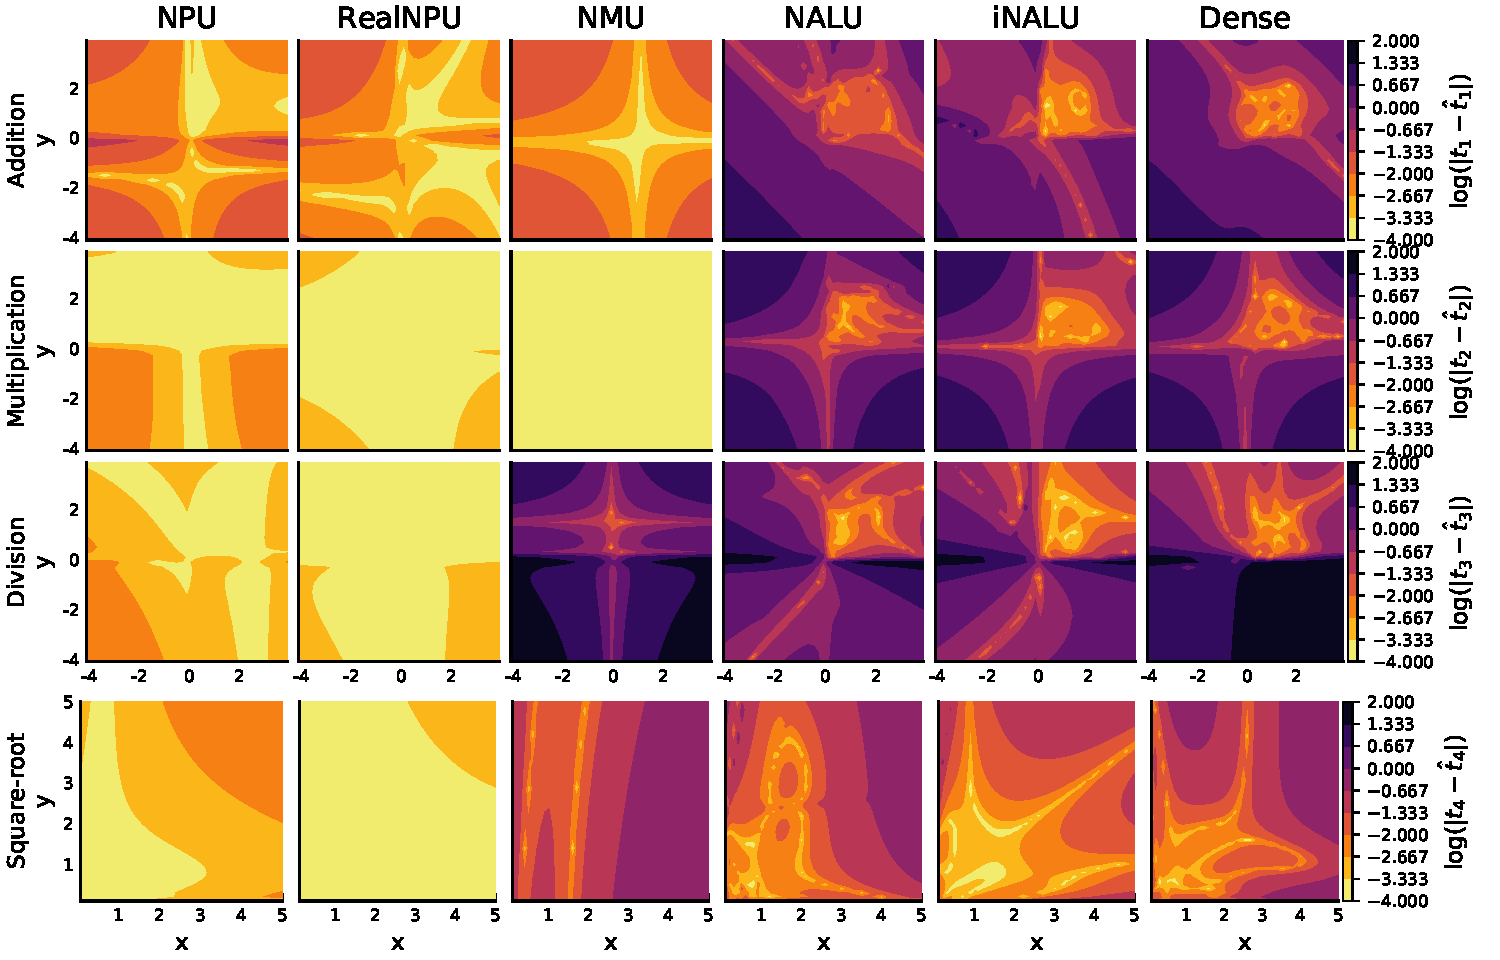
\includegraphics[width=0.9\textwidth]{../plots/simple_err.pdf}
  \end{figure}
  \vspace{-0.6cm}
  \hspace{1cm}
  {\tiny \emph{\bf RealNPU} denotes the NPU with $W_i=0$.
  %\emph{iNALU} is an improved NALU by Schl\"or et al.
  }
\end{frame}

\begin{frame}{Towards Equation Discovery}
  \centering
  The fractional SIR model (fSIR, Taghvaei et al. [2020])
  \begin{equation*}
    \begin{bmatrix}
      \dot S \\ \dot I \\ \dot R
    \end{bmatrix}
    =
    \begin{bmatrix}
      -\beta & 0 & \eta \\
      \beta & -\alpha & 0 \\
      0 & \alpha & \eta
    \end{bmatrix}
    \begin{bmatrix}
      I^\gamma S^\kappa \\ I \\ R
    \end{bmatrix},
    \begin{matrix}
      \alpha=0.05 \\ \beta=0.05 \\ \eta=0.01 \\ \gamma=\kappa=0.5
    \end{matrix}
  \end{equation*}
  \resizebox{.6\textwidth}{!}{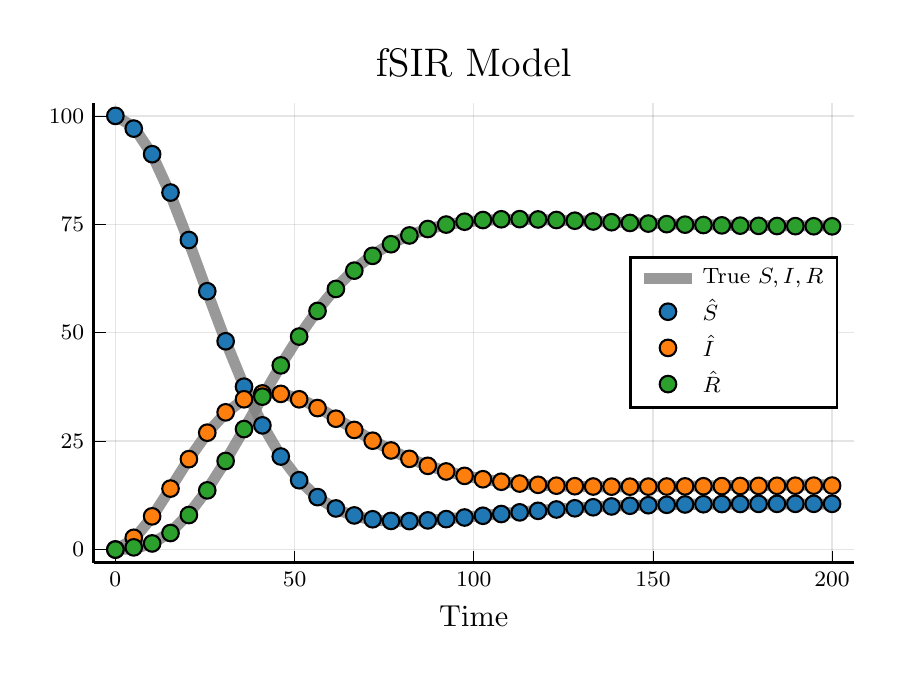
\begin{tikzpicture}[/tikz/background rectangle/.style={fill={rgb,1:red,1.0;green,1.0;blue,1.0}, draw opacity={1.0}}, show background rectangle]
\begin{axis}[point meta max={nan}, point meta min={nan}, legend cell align={left}, title={fSIR Model}, title style={at={{(0.5,1)}}, anchor={south}, font={{\fontsize{14 pt}{18.2 pt}\selectfont}}, color={rgb,1:red,0.0;green,0.0;blue,0.0}, draw opacity={1.0}, rotate={0.0}}, legend style={color={rgb,1:red,0.0;green,0.0;blue,0.0}, draw opacity={1.0}, line width={1}, solid, fill={rgb,1:red,1.0;green,1.0;blue,1.0}, fill opacity={1.0}, text opacity={1.0}, font={{\fontsize{8 pt}{10.4 pt}\selectfont}}, at={(0.98, 0.5)}, anchor={east}}, axis background/.style={fill={rgb,1:red,1.0;green,1.0;blue,1.0}, opacity={1.0}}, anchor={north west}, xshift={115.3mm}, yshift={-1.0mm}, width={112.3mm}, height={74.2mm}, scaled x ticks={false}, xlabel={Time}, x tick style={color={rgb,1:red,0.0;green,0.0;blue,0.0}, opacity={1.0}}, x tick label style={color={rgb,1:red,0.0;green,0.0;blue,0.0}, opacity={1.0}, rotate={0}}, xlabel style={at={(ticklabel cs:0.5)}, anchor=near ticklabel, font={{\fontsize{11 pt}{14.3 pt}\selectfont}}, color={rgb,1:red,0.0;green,0.0;blue,0.0}, draw opacity={1.0}, rotate={0.0}}, xmajorgrids={true}, xmin={-6.0}, xmax={206.0}, xtick={{0.0,50.0,100.0,150.0,200.0}}, xticklabels={{$0$,$50$,$100$,$150$,$200$}}, xtick align={inside}, xticklabel style={font={{\fontsize{8 pt}{10.4 pt}\selectfont}}, color={rgb,1:red,0.0;green,0.0;blue,0.0}, draw opacity={1.0}, rotate={0.0}}, x grid style={color={rgb,1:red,0.0;green,0.0;blue,0.0}, draw opacity={0.1}, line width={0.5}, solid}, axis x line*={left}, x axis line style={color={rgb,1:red,0.0;green,0.0;blue,0.0}, draw opacity={1.0}, line width={1}, solid}, scaled y ticks={false}, ylabel={}, y tick style={color={rgb,1:red,0.0;green,0.0;blue,0.0}, opacity={1.0}}, y tick label style={color={rgb,1:red,0.0;green,0.0;blue,0.0}, opacity={1.0}, rotate={0}}, ylabel style={at={(ticklabel cs:0.5)}, anchor=near ticklabel, font={{\fontsize{11 pt}{14.3 pt}\selectfont}}, color={rgb,1:red,0.0;green,0.0;blue,0.0}, draw opacity={1.0}, rotate={0.0}}, ymajorgrids={true}, ymin={-3.0}, ymax={103.0}, ytick={{0.0,25.0,50.0,75.0,100.0}}, yticklabels={{$0$,$25$,$50$,$75$,$100$}}, ytick align={inside}, yticklabel style={font={{\fontsize{8 pt}{10.4 pt}\selectfont}}, color={rgb,1:red,0.0;green,0.0;blue,0.0}, draw opacity={1.0}, rotate={0.0}}, y grid style={color={rgb,1:red,0.0;green,0.0;blue,0.0}, draw opacity={0.1}, line width={0.5}, solid}, axis y line*={left}, y axis line style={color={rgb,1:red,0.0;green,0.0;blue,0.0}, draw opacity={1.0}, line width={1}, solid}]
    \addplot[color={rgb,1:red,0.502;green,0.502;blue,0.502}, name path={4d2d32cf-0078-477b-aca5-ac47612e3b35}, draw opacity={0.8}, line width={4}, solid]
        coordinates {
            (0.0,100.0)
            (5.128205128205129,97.46721309713212)
            (10.256410256410257,91.07411529978752)
            (15.384615384615385,81.85822003827998)
            (20.512820512820515,70.93406989207153)
            (25.641025641025642,59.36171599653322)
            (30.76923076923077,48.05121932732702)
            (35.8974358974359,37.70386572153941)
            (41.02564102564103,28.786661655619767)
            (46.15384615384615,21.536458098202502)
            (51.282051282051285,15.984367444258964)
            (56.41025641025641,12.000464352759552)
            (61.53846153846154,9.344211354396093)
            (66.66666666666667,7.730064928992786)
            (71.7948717948718,6.871778028659456)
            (76.92307692307692,6.531712440790295)
            (82.05128205128206,6.527846168986343)
            (87.17948717948718,6.732261015727868)
            (92.3076923076923,7.058906461697017)
            (97.43589743589743,7.448852247665159)
            (102.56410256410257,7.8621381580828835)
            (107.6923076923077,8.271957039163652)
            (112.82051282051282,8.660383314615434)
            (117.94871794871794,9.015599814052901)
            (123.07692307692308,9.330728378580337)
            (128.2051282051282,9.603063253817359)
            (133.33333333333334,9.832194944069075)
            (138.46153846153845,10.019480104740795)
            (143.5897435897436,10.168236969594094)
            (148.71794871794873,10.282830242207533)
            (153.84615384615384,10.367552891075434)
            (158.97435897435898,10.42665962038892)
            (164.10256410256412,10.464984481530161)
            (169.23076923076923,10.487122611260277)
            (174.35897435897436,10.496809113024415)
            (179.48717948717947,10.49696822418185)
            (184.6153846153846,10.490486949159731)
            (189.74358974358975,10.479876278697317)
            (194.87179487179486,10.467010848152167)
            (200.0,10.453187053405765)
        }
        ;
    \addlegendentry {True $S,I,R$}
    \addplot[color={rgb,1:red,0.502;green,0.502;blue,0.502}, name path={b32b3689-d920-4aa7-9895-f3013f9b1a1b}, draw opacity={0.8}, line width={4}, solid, forget plot]
        coordinates {
            (0.0,0.01)
            (5.128205128205129,2.326002254590468)
            (10.256410256410257,7.535412858135904)
            (15.384615384615385,14.122344350839555)
            (20.512820512820515,20.861212946319004)
            (25.641025641025642,26.852061199698944)
            (30.76923076923077,31.52079010396936)
            (35.8974358974359,34.589940517583635)
            (41.02564102564103,36.03247808932137)
            (46.15384615384615,36.0106783095002)
            (51.282051282051285,34.81461042142043)
            (56.41025641025641,32.799670718853136)
            (61.53846153846154,30.321886606977262)
            (66.66666666666667,27.70444740533231)
            (71.7948717948718,25.186917212993873)
            (76.92307692307692,22.920167986169474)
            (82.05128205128206,20.97478194912876)
            (87.17948717948718,19.361879697078066)
            (92.3076923076923,18.06136663645284)
            (97.43589743589743,17.0351828644295)
            (102.56410256410257,16.243460467487697)
            (107.6923076923077,15.64716970581006)
            (112.82051282051282,15.209576700999039)
            (117.94871794871794,14.900102701702954)
            (123.07692307692308,14.692768418941395)
            (128.2051282051282,14.564262720391902)
            (133.33333333333334,14.495696710475123)
            (138.46153846153845,14.472242253795276)
            (143.5897435897436,14.480798749993546)
            (148.71794871794873,14.510674957112856)
            (153.84615384615384,14.553801666023665)
            (158.97435897435898,14.60424306180992)
            (164.10256410256412,14.656998699052162)
            (169.23076923076923,14.708526692892267)
            (174.35897435897436,14.75644891382746)
            (179.48717948717947,14.799483648325703)
            (184.6153846153846,14.836795847017735)
            (189.74358974358975,14.868211842226707)
            (194.87179487179486,14.893874068806547)
            (200.0,14.91412562301017)
        }
        ;
    \addplot[color={rgb,1:red,0.502;green,0.502;blue,0.502}, name path={d04156b5-29d1-4f76-8661-f226866e6ee2}, draw opacity={0.8}, line width={4}, solid, forget plot]
        coordinates {
            (0.0,0.0)
            (5.128205128205129,0.21678464827744337)
            (10.256410256410257,1.4004718420766002)
            (15.384615384615385,4.029435610880507)
            (20.512820512820515,8.214717161609485)
            (25.641025641025642,13.796222803767884)
            (30.76923076923077,20.43799056870365)
            (35.8974358974359,27.71619376087699)
            (41.02564102564103,35.19086025505889)
            (46.15384615384615,42.462863592297325)
            (51.282051282051285,49.21102213432063)
            (56.41025641025641,55.20986492838734)
            (61.53846153846154,60.34390203862667)
            (66.66666666666667,64.57548766567494)
            (71.7948717948718,67.95130475834671)
            (76.92307692307692,70.55811957304027)
            (82.05128205128206,72.50737188188494)
            (87.17948717948718,73.9158592871941)
            (92.3076923076923,74.88972690185018)
            (97.43589743589743,75.52596488790537)
            (102.56410256410257,75.90440137442945)
            (107.6923076923077,76.09087325502632)
            (112.82051282051282,76.14003998438557)
            (117.94871794871794,76.09429748424418)
            (123.07692307692308,75.9865032024783)
            (128.2051282051282,75.84267402579079)
            (133.33333333333334,75.68210834545584)
            (138.46153846153845,75.51827764146397)
            (143.5897435897436,75.36096428041239)
            (148.71794871794873,75.21649480067964)
            (153.84615384615384,75.08864544290094)
            (158.97435897435898,74.97909731780119)
            (164.10256410256412,74.8880168194177)
            (169.23076923076923,74.81435069584748)
            (174.35897435897436,74.75674197314815)
            (179.48717948717947,74.71354812749247)
            (184.6153846153846,74.68271720382256)
            (189.74358974358975,74.661911879076)
            (194.87179487179486,74.64911508304131)
            (200.0,74.6426873235841)
        }
        ;
    \addplot[color={rgb,1:red,0.1216;green,0.4667;blue,0.7059}, name path={daf90f21-20cf-4381-9c0f-30de95c3d54b}, draw opacity={1.0}, line width={0}, solid, mark={*}, mark size={3.0 pt}, mark options={color={rgb,1:red,0.0;green,0.0;blue,0.0}, draw opacity={1.0}, fill={rgb,1:red,0.1216;green,0.4667;blue,0.7059}, fill opacity={1.0}, line width={0.75}, rotate={0}, solid}, only marks]
        coordinates {
            (0.0,100.0)
            (5.128205128205129,97.06371891032103)
            (10.256410256410257,91.16684462650328)
            (15.384615384615385,82.31860705364566)
            (20.512820512820515,71.37328028612147)
            (25.641025641025642,59.56655329185587)
            (30.76923076923077,48.02982853680665)
            (35.8974358974359,37.56283706154292)
            (41.02564102564103,28.637211640920665)
            (46.15384615384615,21.450945359433096)
            (51.282051282051285,15.991646351608207)
            (56.41025641025641,12.091156352995037)
            (61.53846153846154,9.484490451837605)
            (66.66666666666667,7.875556914992195)
            (71.7948717948718,6.990870233379205)
            (76.92307692307692,6.607983321954687)
            (82.05128205128206,6.5600222783518465)
            (87.17948717948718,6.726996153400294)
            (92.3076923076923,7.024919064760524)
            (97.43589743589743,7.39470727063654)
            (102.56410256410257,7.794775985610217)
            (107.6923076923077,8.196178604628553)
            (112.82051282051282,8.579336543097728)
            (117.94871794871794,8.931747895191842)
            (123.07692307692308,9.246307992466145)
            (128.2051282051282,9.520025067810243)
            (133.33333333333334,9.752717909881044)
            (138.46153846153845,9.946211973122255)
            (143.5897435897436,10.103649973188396)
            (148.71794871794873,10.228936301333658)
            (153.84615384615384,10.326310541375907)
            (158.97435897435898,10.400033334390523)
            (164.10256410256412,10.454186099682712)
            (169.23076923076923,10.492511634963721)
            (174.35897435897436,10.518286052520692)
            (179.48717948717947,10.534341485628904)
            (184.6153846153846,10.543067590956252)
            (189.74358974358975,10.546434143372755)
            (194.87179487179486,10.546027918810093)
            (200.0,10.54309740549285)
        }
        ;
    \addlegendentry {$\hat S$}
    \addplot[color={rgb,1:red,1.0;green,0.498;blue,0.0549}, name path={d719ac49-0b45-4546-885d-0971ecba6177}, draw opacity={1.0}, line width={0}, solid, mark={*}, mark size={3.0 pt}, mark options={color={rgb,1:red,0.0;green,0.0;blue,0.0}, draw opacity={1.0}, fill={rgb,1:red,1.0;green,0.498;blue,0.0549}, fill opacity={1.0}, line width={0.75}, rotate={0}, solid}, only marks]
        coordinates {
            (0.0,0.01)
            (5.128205128205129,2.7125599630590216)
            (10.256410256410257,7.66090322551522)
            (15.384615384615385,14.05992089552267)
            (20.512820512820515,20.853377037596527)
            (25.641025641025642,26.949263303743713)
            (30.76923076923077,31.643268521967897)
            (35.8974358974359,34.65445060429321)
            (41.02564102564103,36.00248493995587)
            (46.15384615384615,35.89734765592843)
            (51.282051282051285,34.65263524249474)
            (56.41025641025641,32.62658545846643)
            (61.53846153846154,30.171255479960887)
            (66.66666666666667,27.588258250205744)
            (71.7948717948718,25.101967545018532)
            (76.92307692307692,22.854404251300224)
            (82.05128205128206,20.916574933981376)
            (87.17948717948718,19.306505476039106)
            (92.3076923076923,18.00963924091414)
            (97.43589743589743,16.993337294186258)
            (102.56410256410257,16.217140779474875)
            (107.6923076923077,15.639502083735772)
            (112.82051282051282,15.2216338588409)
            (117.94871794871794,14.929362607150622)
            (123.07692307692308,14.733677548787432)
            (128.2051282051282,14.610599644370984)
            (133.33333333333334,14.541013265661315)
            (138.46153846153845,14.509771044572922)
            (143.5897435897436,14.505057091871647)
            (148.71794871794873,14.517816285691135)
            (153.84615384615384,14.541245312235125)
            (158.97435897435898,14.570351813286242)
            (164.10256410256412,14.601580037074164)
            (169.23076923076923,14.632505354378589)
            (174.35897435897436,14.661561456708021)
            (179.48717948717947,14.687819457461144)
            (184.6153846153846,14.710818905225636)
            (189.74358974358975,14.730432472745509)
            (194.87179487179486,14.746759324518035)
            (200.0,14.760042741576434)
        }
        ;
    \addlegendentry {$\hat I$}
    \addplot[color={rgb,1:red,0.1725;green,0.6275;blue,0.1725}, name path={209e1cdb-c150-414a-bfc5-63b07ba91f51}, draw opacity={1.0}, line width={0}, solid, mark={*}, mark size={3.0 pt}, mark options={color={rgb,1:red,0.0;green,0.0;blue,0.0}, draw opacity={1.0}, fill={rgb,1:red,0.1725;green,0.6275;blue,0.1725}, fill opacity={1.0}, line width={0.75}, rotate={0}, solid}, only marks]
        coordinates {
            (0.0,0.0)
            (5.128205128205129,0.50693326871289)
            (10.256410256410257,1.417679355799354)
            (15.384615384615385,3.8182491876122566)
            (20.512820512820515,7.962302503151513)
            (25.641025641025642,13.649388710326537)
            (30.76923076923077,20.427370387367066)
            (35.8974358974359,27.787946129597962)
            (41.02564102564103,35.263551206919445)
            (46.15384615384615,42.46863602460634)
            (51.282051282051285,49.116287047058584)
            (56.41025641025641,55.02090402143257)
            (61.53846153846154,60.09164848079044)
            (66.66666666666667,64.31440131855449)
            (71.7948717948718,67.72832791710991)
            (76.92307692307692,70.40495950573064)
            (82.05128205128206,72.43348328533506)
            (87.17948717948718,73.91170893256104)
            (92.3076923076923,74.93627783745409)
            (97.43589743589743,75.5987646759572)
            (102.56410256410257,75.98223718673248)
            (107.6923076923077,76.15882412766837)
            (112.82051282051282,76.18868881450685)
            (117.94871794871794,76.12017219498782)
            (123.07692307692308,75.99077303726688)
            (128.2051282051282,75.8285172837301)
            (133.33333333333334,75.65344697694208)
            (138.46153846153845,75.47937800364895)
            (143.5897435897436,75.31528402015716)
            (148.71794871794873,75.16647568233809)
            (153.84615384615384,75.03557984442344)
            (158.97435897435898,74.92332819239051)
            (164.10256410256412,74.82915576306749)
            (169.23076923076923,74.75168343757129)
            (174.35897435897436,74.68913253538693)
            (179.48717948717947,74.63952887626489)
            (184.6153846153846,74.60087490919402)
            (189.74358974358975,74.57126520497009)
            (194.87179487179486,74.54895766923063)
            (200.0,74.53241178440281)
        }
        ;
    \addlegendentry {$\hat R$}
\end{axis}
\end{tikzpicture}
}
\end{frame}

\begin{frame}{Towards Equation Discovery}
  \centering
  The fractional SIR model (fSIR, Taghvaei et al. [2020])
  \begin{equation*}
    \begin{bmatrix}
      \dot S \\ \dot I \\ \dot R
    \end{bmatrix}
    =
    \begin{bmatrix}
      -\beta & 0 & \eta \\
      \beta & -\alpha & 0 \\
      0 & \alpha & \eta
    \end{bmatrix}
    \begin{bmatrix}
      I^\gamma S^\kappa \\ I \\ R
    \end{bmatrix},
    \begin{matrix}
      \alpha=0.05 \\ \beta=0.05 \\ \eta=0.01 \\ \gamma=\kappa=0.5
    \end{matrix}
  \end{equation*}
  \begin{figure}
    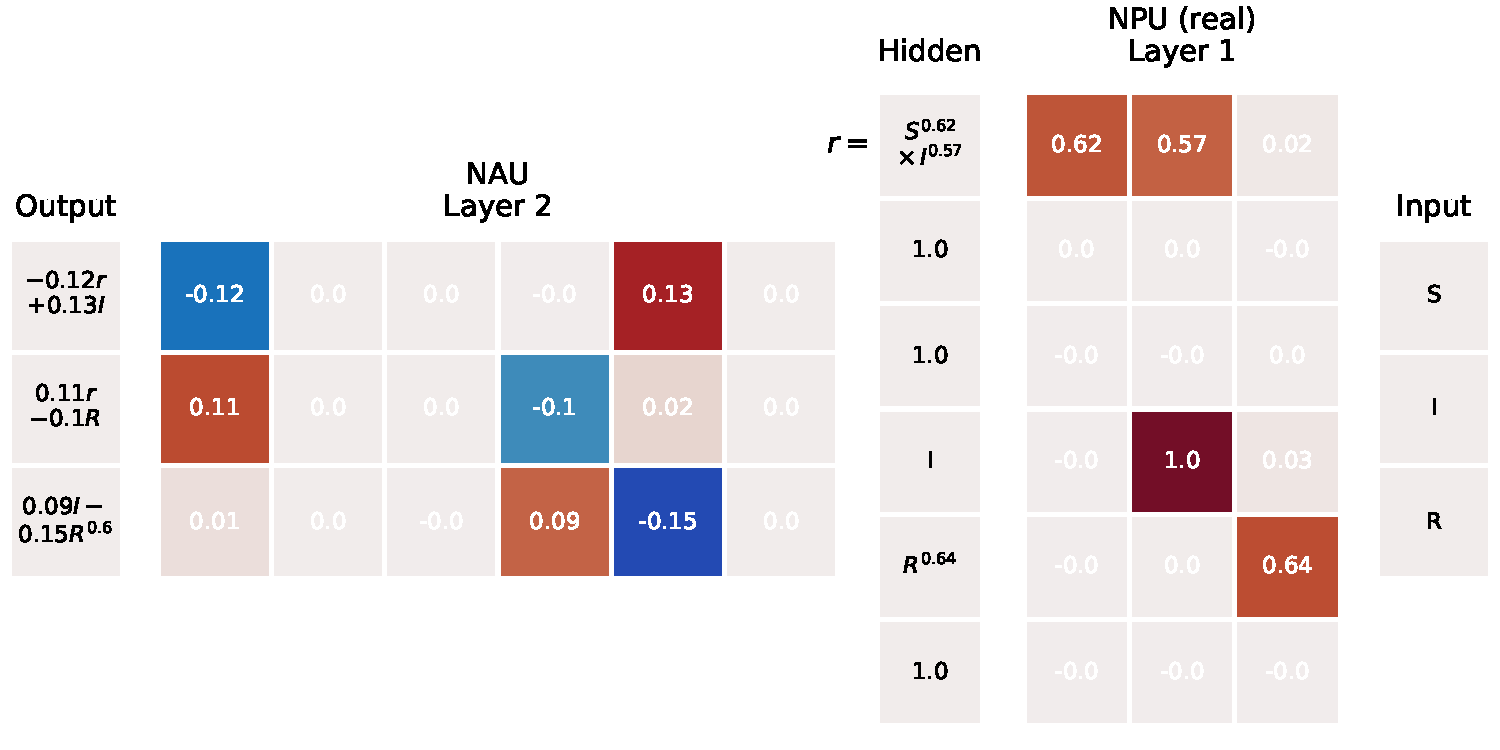
\includegraphics[width=0.8\linewidth]{../plots/sir_gatednpu_modelps.pdf}
  \end{figure}
  \vspace{-1.5cm}
  \hspace{-4cm}
  {\tiny *Trained with $L_1$-reg. to achieve sparse results.}
\end{frame}

\maketitle

\end{document}
